\documentclass[11pt]{article}

% --- Page layout ---
\usepackage[a4paper,margin=2cm]{geometry}

% --- Typography and section formatting ---
\usepackage{parskip} % Adds space between paragraphs
\usepackage{titlesec} % Custom section formatting
\titleformat{\section}{\normalfont\Large\bfseries}{}{0pt}{}
\titleformat{\subsection}{\normalfont\large\bfseries}{}{0pt}{}

% --- Math and symbols ---
\usepackage{amsmath} % For math environments

% --- Figures and tables ---
\usepackage{graphicx} % For including graphics
\usepackage{float} % For figure placement
\usepackage{caption} % For customizing captions
\usepackage{subcaption} % For subfigures
\captionsetup[figure]{justification=centering, font=small, skip=4pt}
\usepackage{booktabs} % Nicer tables
\usepackage{array} % Extended table formatting
\newcolumntype{M}[1]{>{\centering\arraybackslash}m{#1}} % Centered column type

% --- URLs and hyperlinks ---
\usepackage{url} % For URL formatting

% --- Document starts here ---
\begin{document}
	
	\begin{center}
		\LARGE\textbf{Bayesian Spatial Risk Modelling of Suicide Mortality in South Korea}
	\end{center}
	
	\section*{1. Background}
	
	South Korea consistently reports one of the highest suicide rates among developed nations, with 24 to 28 deaths per 100,000 people in recent years—more than twice the OECD average of 11 (Kim, 2024). This persistent trend positions South Korea as a global outlier and underscores the urgent need to investigate its underlying risk factors. Classical theories dating back to Durkheim (1951) emphasise the protective role of social integration, while recognising economic hardship and mental illness as key drivers of suicide. In South Korea, national crises such as the late-1990s Asian financial crash have been linked to suicide spikes, primarily through rising unemployment and social dislocation (Chang, 2009).
	
	Four key factors have been linked to elevated suicide risk in South Korea: social isolation, psychological stress, unemployment, and unmet medical needs. Areas with more single-person households or divorced residents tend to report higher suicide rates, with higher rates observed in areas with weaker social ties (Jang, 2022). High levels of perceived stress, measured through the “stress awareness” indicator, are associated with depression, suicidal ideation, and increased regional suicide rates (Oh, 2020). Unemployment contributes to financial strain and psychological distress, and its association with higher suicide rates is particularly evident where social safety nets are weak (Park \& Lester, 2006). Lastly, unmet medical needs—reflecting limited healthcare access—are correlated with higher suicide mortality, with only about 15\% of affected individuals receiving treatment despite the high prevalence of mental health conditions (Kim, 2022).
	
	This study employs a Bayesian Intrinsic Conditional Auto-Regressive (ICAR) model to estimate spatial variation in suicide risk across South Korea, using the four covariates above. Key outputs include localised estimates of relative risk and global regression coefficients, providing an evidence base to support public health interventions and regional resource allocation.

	\section*{2. Data and Methods}
	
	\subsection*{2.1 Study Area}	
	
	The study area encompasses all 229 municipalities in South Korea, including cities (\textit{shi}), counties (\textit{kun}), and districts (\textit{ku}), collectively referred to as \textit{shikunku}-level administrative units. This spatial resolution was selected as it represents the most granular level at which all covariates are consistently available and corresponds to the administrative scale at which suicide prevention policies are typically developed and implemented. Spatial boundaries were derived from official 2022 shapefiles, to which all statistical datasets were harmonised by resolving naming inconsistencies, aggregating sub-municipal divisions, and reversing backdated administrative updates. To ensure full connectivity in the Queen contiguity adjacency matrix, disconnected island polygons were linked to the mainland subgraph using nearest-neighbour centroids.
	
	\subsection*{2.2 Data}
	
	The primary outcome variable is the estimated number of \textit{shikunku}-level suicide deaths in 2022. This was calculated by multiplying the age-standardised suicide rate (per 100,000 people) by the mid-year population for each municipality. Suicide rates were obtained from Statistics Korea’s \textit{Cause of Death Statistics}, while population estimates originate from the 2022 \textit{Future Population Projections}.
		
	Four predictor variables were selected based on their relevance in the literature: the single-person household ratio, stress awareness rate, unemployment rate, and unmet medical needs rate. All variables reflect conditions in 2022 and were obtained from national databases, as summarised in Table~\ref{tab:datasets}. Figure~\ref{fig:suicide_map_2022} provides a visual overview of suicide rates across the country.
	
	\begin{table}[H]
		\centering
		\caption{Summary of Datasets}
		\renewcommand{\arraystretch}{1.4}
		\resizebox{\textwidth}{!}{%
			\begin{tabular}{M{4.5cm} M{4.5cm} M{3.5cm} M{5cm} M{1.2cm}}
				\toprule
				\textbf{Variable} & \textbf{Dataset} & \textbf{Usage} & \textbf{Source} & \textbf{Year} \\
				\midrule
				\textbf{Suicide Rate} & Cause of Death Statistics & Target variable & Statistics Korea (Population Trends Division) & 2022 \\
				\textbf{Single-Person Household Ratio} & Population and Housing Census & Predictor variable & Statistics Korea (Population and Housing Census Division) & 2022 \\
				\textbf{Stress Awareness Rate} & Community Health Survey & Predictor variable & Korea Disease Control and Prevention Agency (KDCA) & 2022 \\
				\textbf{Unemployment Rate} & Local Employment Statistics & Predictor variable & Statistics Korea (Employment Statistics Division) & 2022 \\
				\textbf{Unmet Medical Needs Rate} & Community Health Survey & Predictor variable & Korea Disease Control and Prevention Agency (KDCA) & 2022 \\
				\textbf{Estimated Population} & Future Population Projections & Standardisation / Denominator & Statistics Korea (Regional Statistics Planning Division) & 2022 \\
				\textbf{Municipality Boundaries} & Municipality Shapefiles & Spatial analysis & Statistical Geographic Information System (SGIS) & 2022 \\
				\textbf{Province Boundaries} & Province Shapefiles & Mapping / Labelling & Statistical Geographic Information System (SGIS) & 2022 \\
				\bottomrule
			\end{tabular}
		}
		\label{tab:datasets}
	\end{table}
	
	\begin{figure}[H]
		\centering
		\caption{Suicide Rates Across Municipalities}
		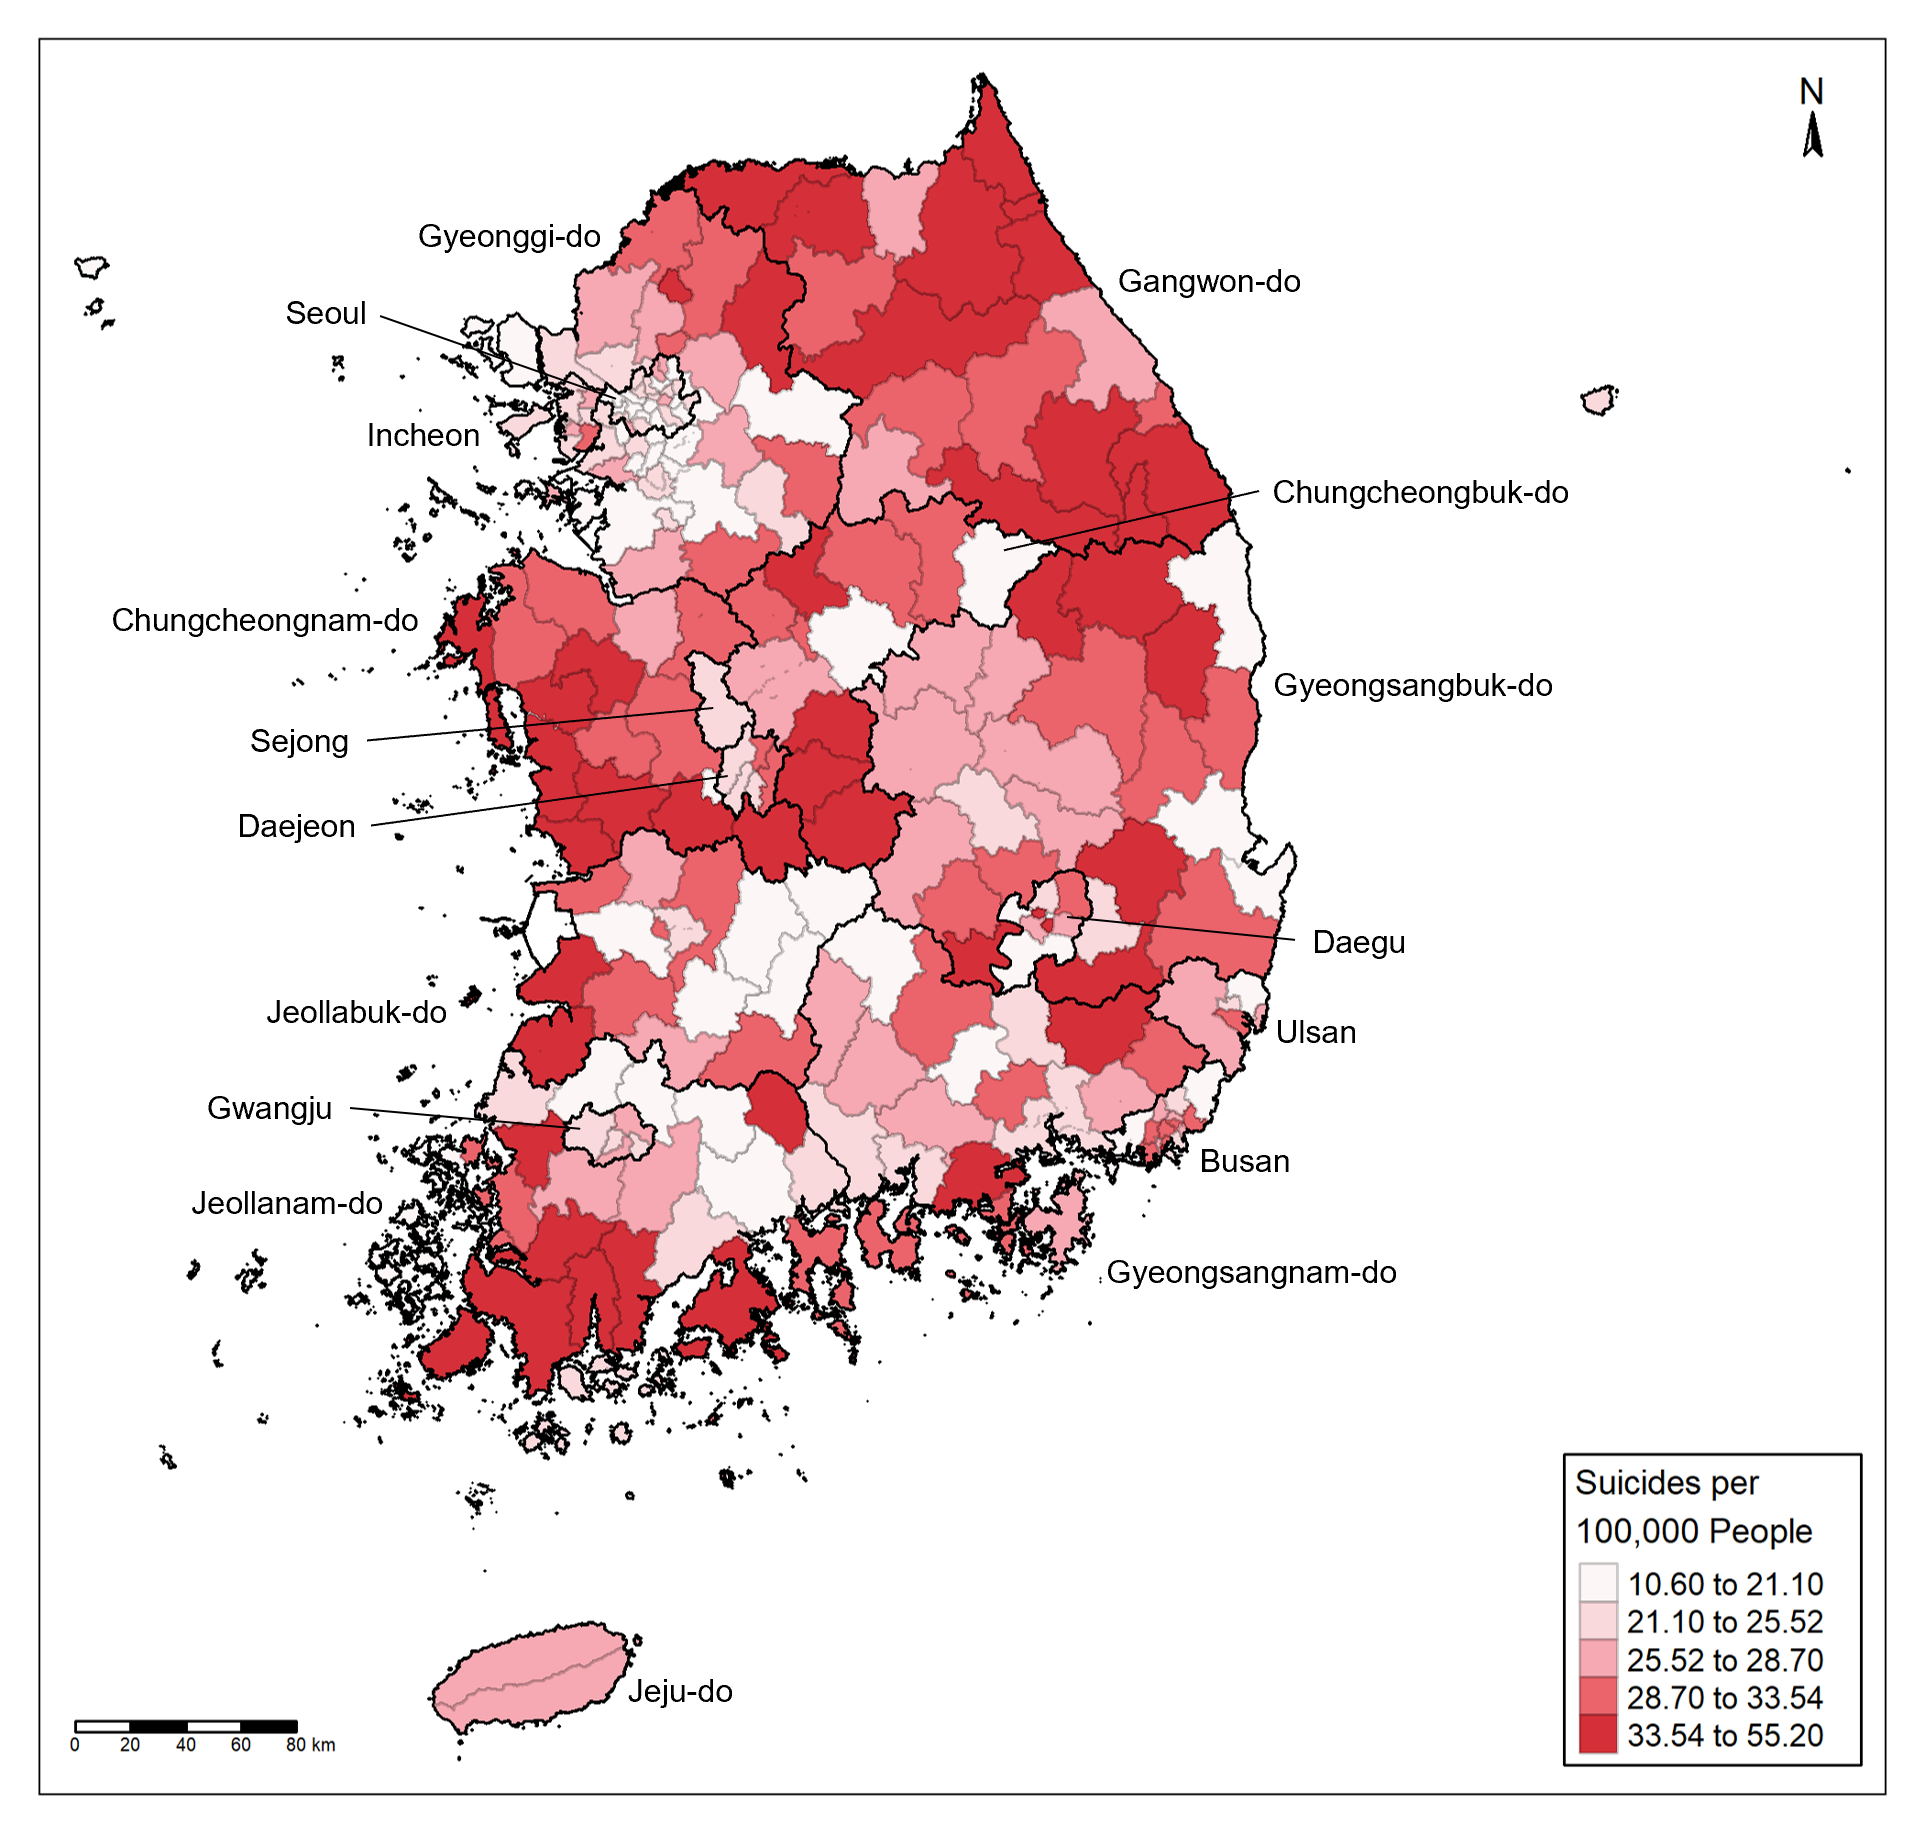
\includegraphics[width=0.8\textwidth]{assets/suicide_map/suicide_map_2022_annotated.png}
		\label{fig:suicide_map_2022}
	\end{figure}
	
	\newpage
	\subsection*{2.3 Methods}
	
	We employed a Bayesian Poisson regression model with spatial effects to estimate the relative risk (RR) of suicide mortality across South Korean municipalities. To account for spatial autocorrelation among neighbouring areas, a structured spatial random effect was included using an intrinsic conditional autoregressive (ICAR) prior (Besag, 1991), a standard approach in spatial epidemiology. An unstructured random effect was also added to capture residual heterogeneity not explained by spatial structure or covariates.
	
	The model assumes a Poisson likelihood with a log link and a population-based offset, which is appropriate for modelling rare event counts in small-area epidemiological studies. Spatial adjacency was defined using Queen contiguity, where municipalities sharing either a boundary or vertex were considered neighbours.

	\begin{equation}
		Y_i \sim \text{Poisson}(\lambda_i), \quad 
		\log(\lambda_i) = \log(E_i) + \alpha + \mathbf{X}_i \boldsymbol{\beta} + \sigma \cdot \phi_i\footnote{In the full model, we include both structured and unstructured random effects: 
			$\log(\lambda_i) = \log(E_i) + \alpha + \mathbf{X}_i \boldsymbol{\beta} + \sigma \cdot \left( \sqrt{1 - \rho} \, \theta_i + \sqrt{\rho} \, \phi_i \right)$, where $\theta_i \sim \mathcal{N}(0,1)$ captures unstructured heterogeneity and $\phi_i$ follows an ICAR prior for spatial structure.}
	\end{equation}
	
	Where $Y_i$ denotes the observed number of suicide deaths, $E_i$ the expected count based on population size, $\alpha$ the intercept, $\mathbf{X}_i$ the vector of covariates for municipality $i$, $\boldsymbol{\beta}$ the corresponding coefficients, and $\phi_i$ the spatial random effect scaled by $\sigma$. Structured ($\phi_i$) and unstructured ($\theta_i$) effects are combined through a weighted average governed by $\rho$.
	
	We specified the following priors:
	
	\vspace{1em}
	
	\begin{itemize}
		\item $\alpha \sim \mathcal{N}(0, 1)$ \hfill \textit{(intercept)}
		\item $\boldsymbol{\beta} \sim \mathcal{N}(0, 1)$ \hfill \textit{(covariate coefficients)}
		\item $\theta_i \sim \mathcal{N}(0, 1)$ \hfill \textit{(unstructured random effects)}
		\item $\phi \sim \text{ICAR}(N, \texttt{node1}, \texttt{node2})$ \hfill \textit{(structured spatial random effects)}
		\item $\textstyle \sum_{i=1}^N \phi_i \sim \mathcal{N}(0, 0.001 \cdot N)$ \hfill \textit{(sum-to-zero constraint on $\phi$ to ensure identifiability)}
		\item $\sigma \sim \mathcal{N}(0, 1)$ \hfill \textit{(scaling factor for spatial effects)}
		\item $\rho \sim \text{Beta}(0.5, 0.5)$ \hfill \textit{(mixing proportion between structured and unstructured effects)}
	\end{itemize}
	
	\vspace{1em}
	
	All priors were weakly informative, centred around zero to regularise estimates while allowing flexibility to reflect uncertainty without dominating the posterior. Model fitting was performed in \textit{Stan} using the \textit{rstan} interface in R. We ran six parallel chains with 20,000 iterations each (10,000 warm-up), using the No-U-Turn Sampler (NUTS) with a maximum tree depth of 12.
	
	\newpage
	\section*{3. Results and Discussion}
	
	\subsection*{3.1 Global Parameter Estimates}
	
	\begin{table}[H]
		\centering
		\caption{Posterior Estimates of Global Parameters}
		\renewcommand{\arraystretch}{1.3}
		\begin{tabular}{cccccccc}
			\hline
			\textbf{Parameter} & \textbf{Mean} & \textbf{SE Mean} & \textbf{2.5\% CrI} & \textbf{97.5\% CrI} & \boldmath{$n_\text{eff}$} & \boldmath{$\hat{R}$} \\
			\hline
			$\alpha$   & $-0.1956$ & $0.0008$ & $-0.4548$ & $0.0685$ & $25689.1$ & $1.0005$ \\
			$\beta_1$  & $0.0120$  & $0.0000$ & $0.0067$  & $0.0174$ & $27152.2$ & $1.0003$ \\
			$\beta_2$  & $-0.0052$ & $0.0000$ & $-0.0139$ & $0.0035$ & $26780.3$ & $1.0001$ \\
			$\beta_3$  & $-0.0385$ & $0.0002$ & $-0.0706$ & $-0.0065$ & $9776.5$  & $1.0007$ \\
			$\beta_4$  & $0.0089$  & $0.0000$ & $-0.0014$ & $0.0190$ & $28092.1$ & $1.0001$ \\
			$\sigma$   & $0.2118$  & $0.0003$ & $0.1611$  & $0.2685$ & $7507.3$  & $1.0006$ \\
			\hline
		\end{tabular}
		
		\vspace{0.5em}
		
		\begin{minipage}{0.9\textwidth}
			\vspace{0.5em}
			\footnotesize
			\textit{Note.} SE Mean = Standard Error of Posterior Mean; CrI = Credible Interval; $n_\text{eff}$ indicates the effective sample size. $\hat{R}$ is the Gelman–Rubin convergence diagnostic, where values near 1.00 suggest good convergence.
		\end{minipage}
		\label{tab:icar_results}
	\end{table}
	
	The model converged successfully with all $\hat{R}$ values below 1.05 and large effective sample sizes, indicating stable posterior estimates. The global intercept ($\alpha = -0.20$) corresponds to a relative risk (RR) of $\exp(-0.20) \approx 0.82$ (95\% CrI: 0.63 to 1.07), suggesting slightly lower-than-expected baseline suicide risk. However, the result is not statistically significant, as the credible interval includes the null value of 1.00.
	
	Among the covariates, the unemployment rate ($\beta_3$) showed the strongest and statistically significant association: a one-unit increase corresponds to a 4\% decrease in suicide risk ($RR \approx 0.96$; 95\% CrI: 0.93 to 0.99). The single-person household ratio ($\beta_1$) and unmet medical needs rate ($\beta_4$) had weak positive associations ($RR \approx 1.01$), but their credible intervals approached or included 1.00, indicating limited significance. Stress awareness ($\beta_2$) was negatively associated with suicide risk ($RR \approx 0.99$) but was not statistically significant.
	
	The spatial standard deviation ($\sigma = 0.21$) indicates a meaningful level of spatial heterogeneity, supporting the inclusion of structured spatial effects in the model.
	
	\newpage
	\subsection*{3.2 Spatial Distribution of Relative Risk}

	\vspace{-1em}

	\begin{figure}[H]
		\centering
		\caption{Map of Relative Risk Ratios}
		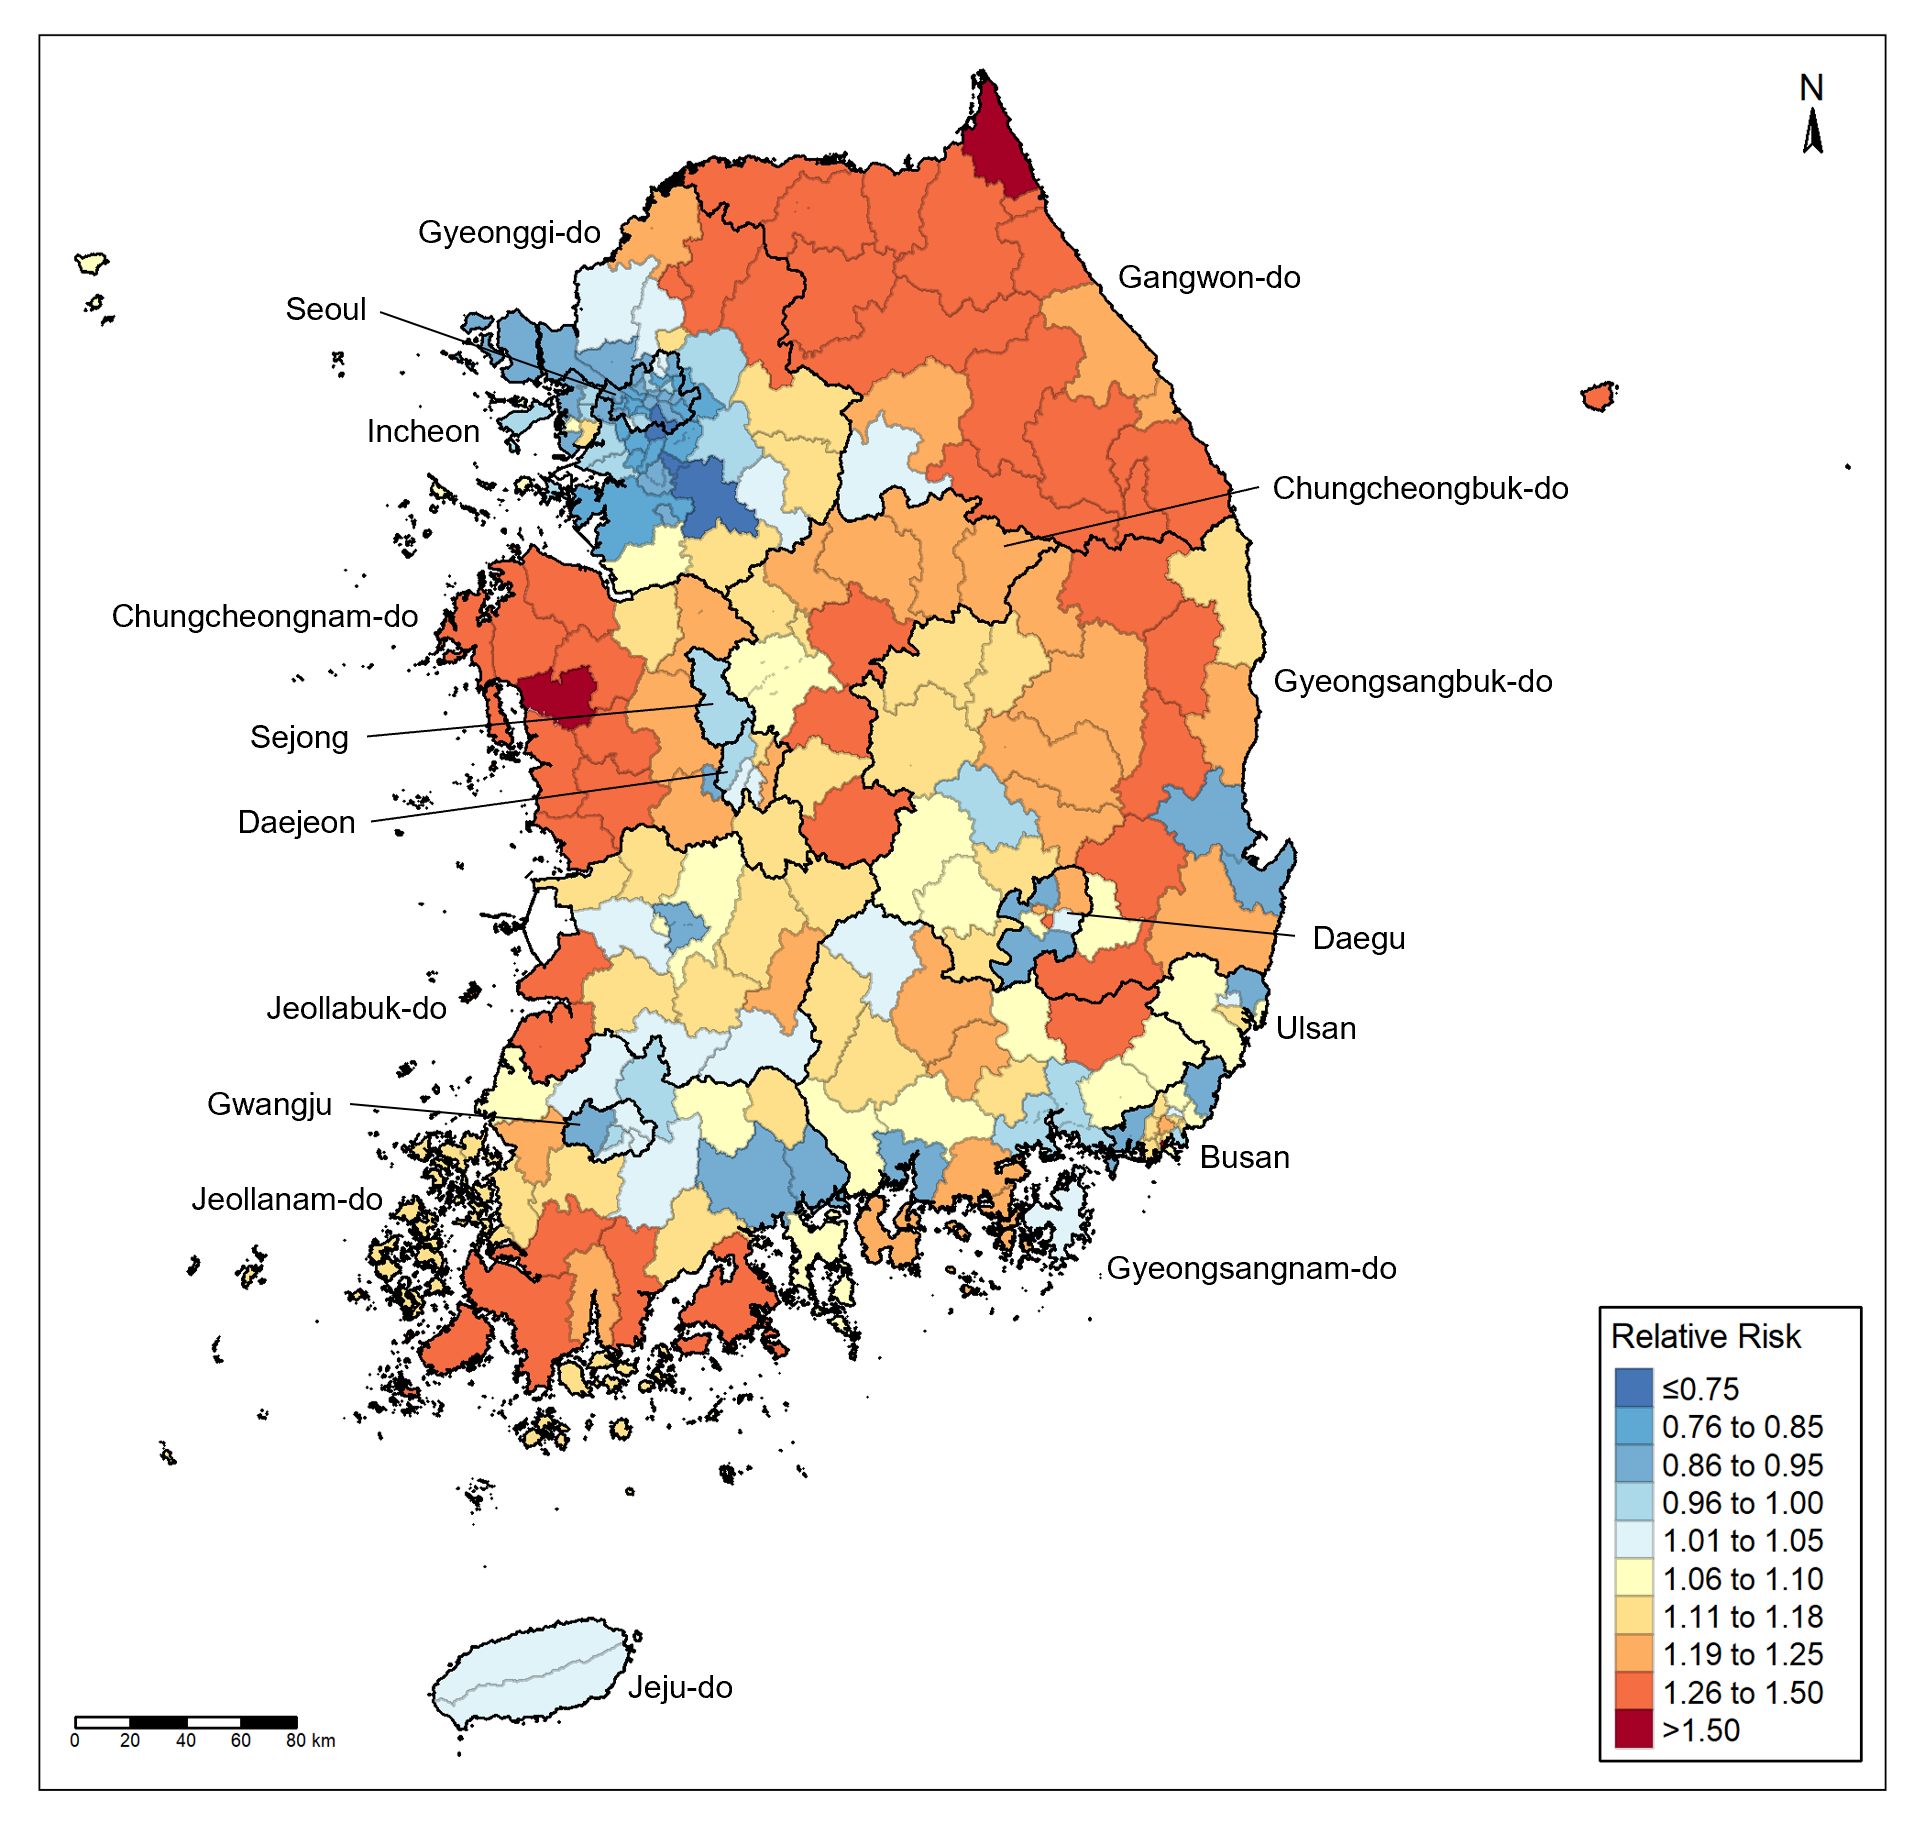
\includegraphics[width=0.74\textwidth]{assets/relative_risk/relative_risk_map_2022_annotated.png}
		\label{fig:relative_risk_map}
	\end{figure}

	\vspace{-2em}
	
	\begin{figure}[H]
		\centering
		\caption{Map of Statistical Significance}
		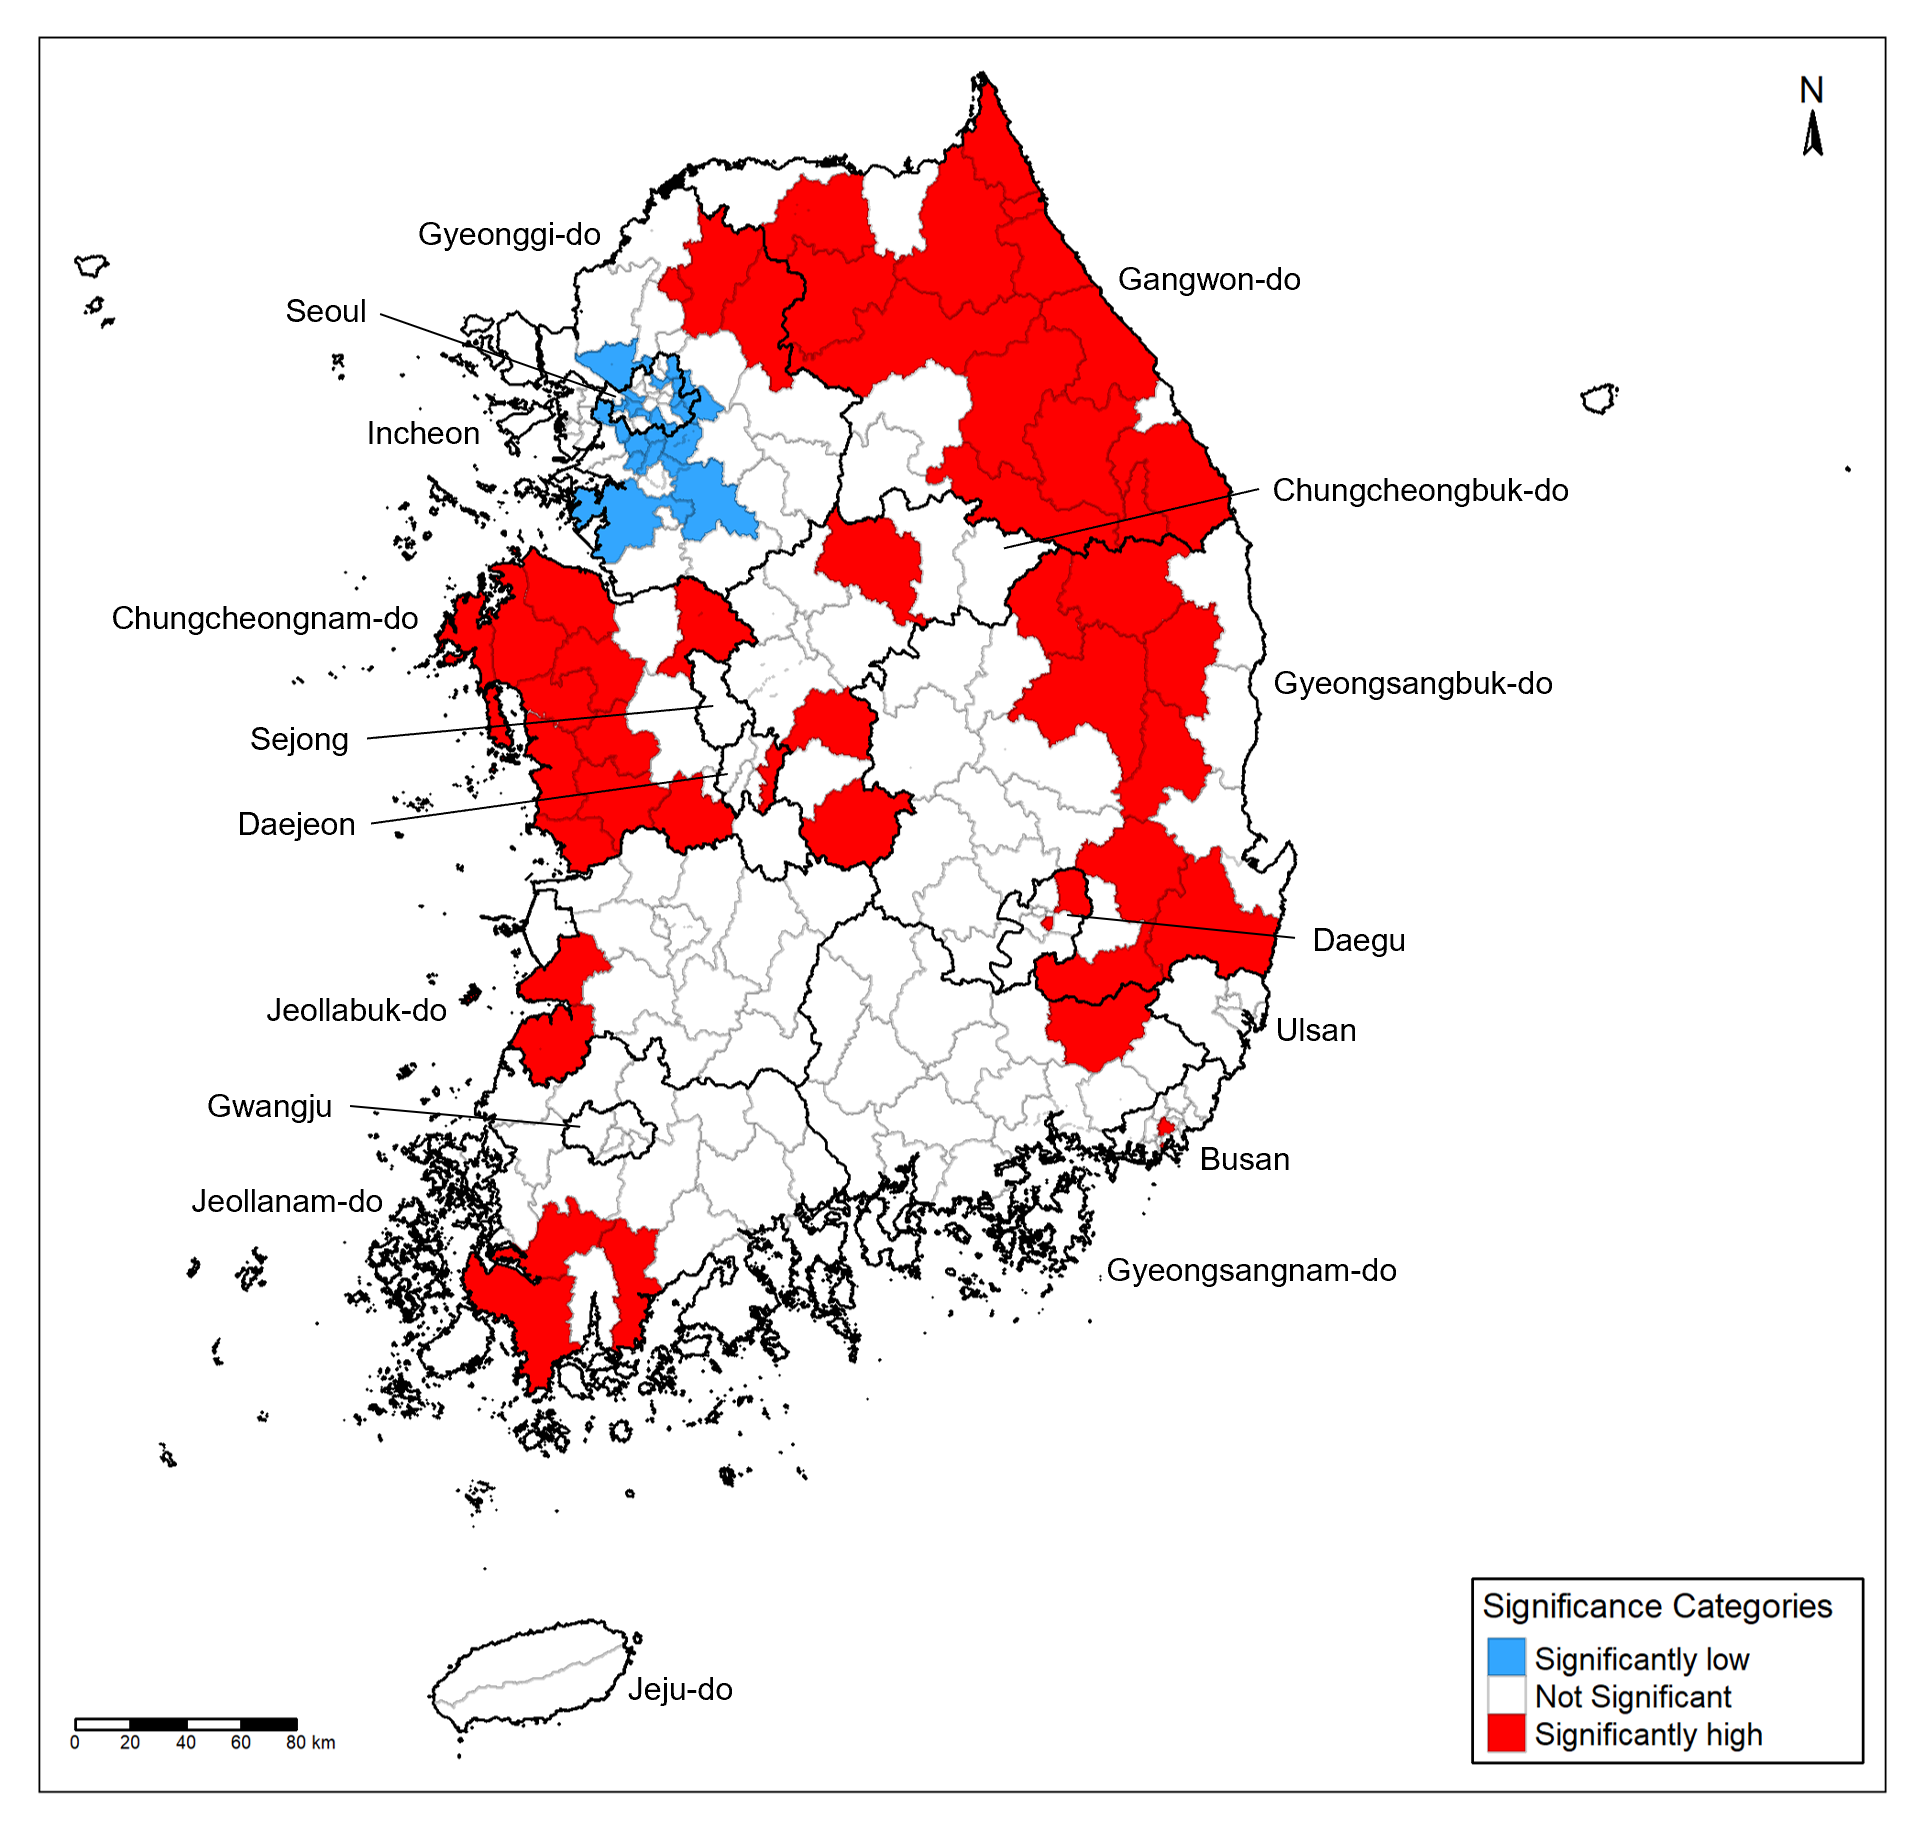
\includegraphics[width=0.74\textwidth]{assets/significance_categories/significance_categories_map_2022_annotated.png}
		\label{fig:significance_map}
	\end{figure}

	\vspace{-2em}
	
	\begin{figure}[H]
		\centering
		\caption{Map of Exceedance Probabilities}
		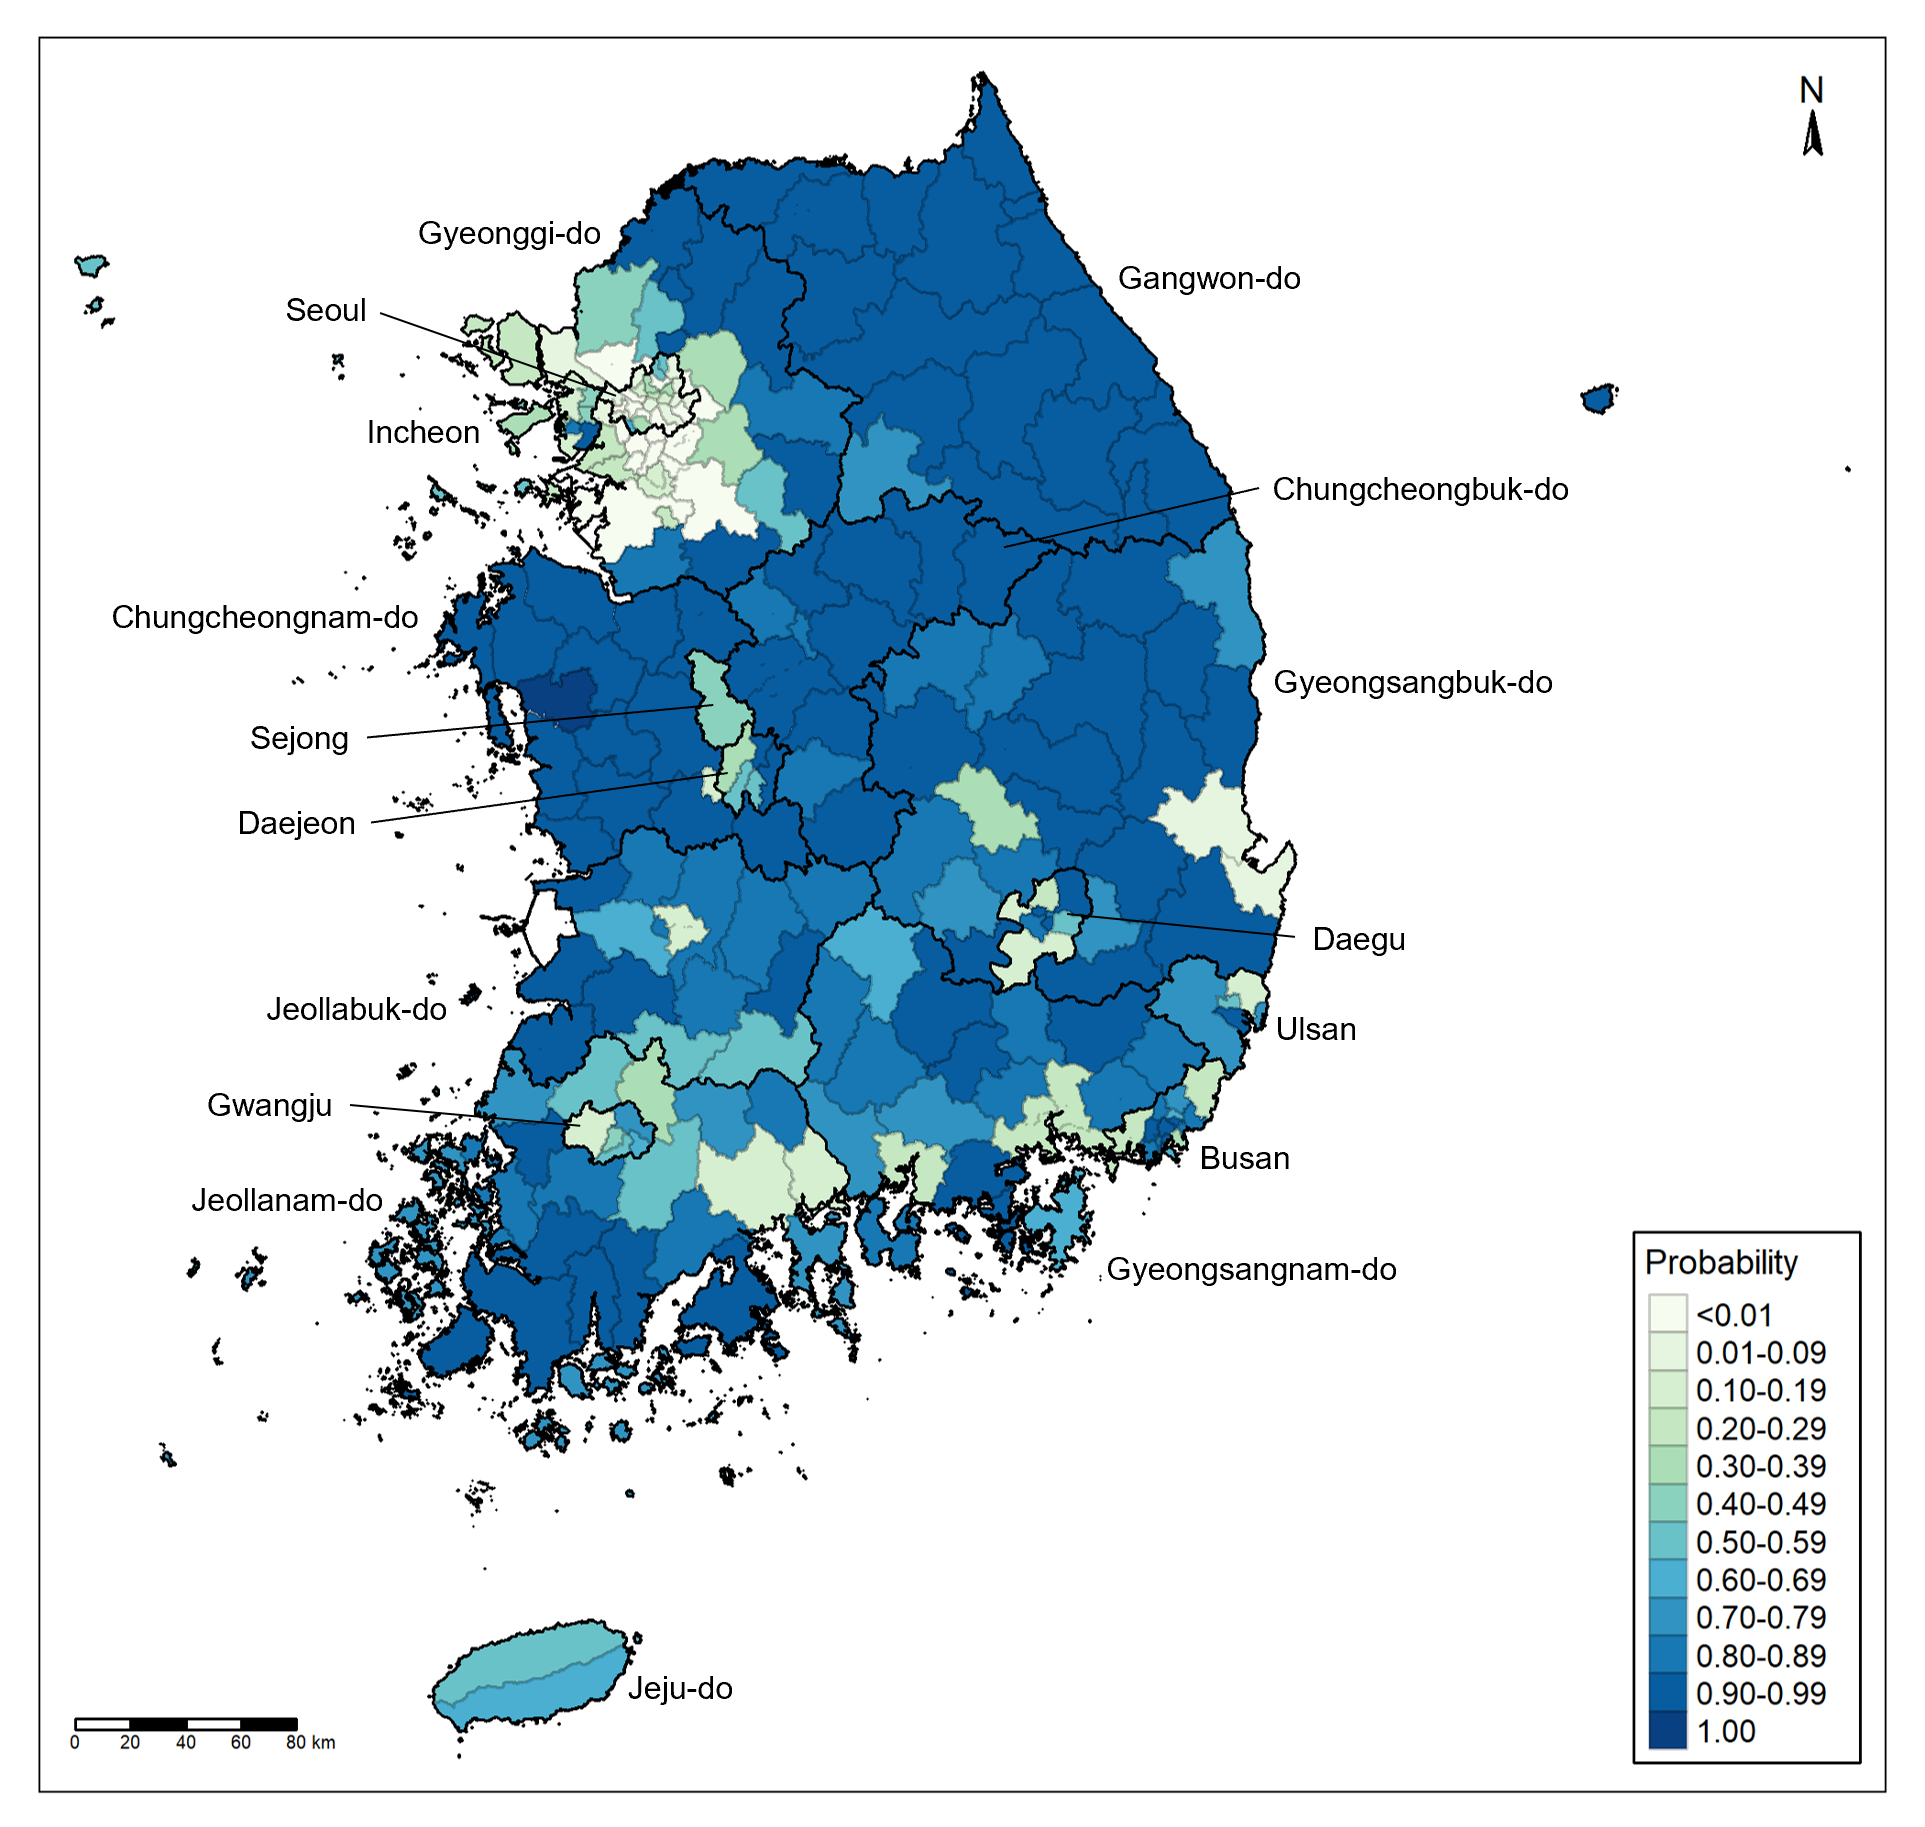
\includegraphics[width=0.74\textwidth]{assets/exceedance_probabilities/exceedance_probabilities_map_2022_annotated.png}
		\label{fig:exceedance_probabilities_map}
	\end{figure}
	
	Figures~\ref{fig:relative_risk_map}, \ref{fig:significance_map}, and \ref{fig:exceedance_probabilities_map} collectively illustrate marked spatial disparities in suicide risk across South Korean municipalities. High-risk areas (RR > 1.25) are prominently clustered in rural regions, particularly in Chungcheongnam-do and Gangwon-do, with some municipalities exceeding an RR of 1.50. These areas are often characterised by limited access to healthcare, economic vulnerability, and higher proportions of older and male residents—demographics typically associated with elevated suicide risk.
	
	In contrast, most low-risk areas (RR < 1.00) are concentrated in urban regions, particularly within the Seoul Metropolitan Area and major cities such as Busan and Daegu. These areas may benefit from stronger healthcare infrastructure, greater economic opportunity, and denser social networks. The clear clustering of high- and low-risk values indicates substantial spatial autocorrelation, underscoring a pronounced urban–rural divide in suicide risk.

	The statistical significance of relative risk estimates further reinforces this pattern. Red municipalities (95\% CrI > 1.00), indicating significantly elevated risk, are predominantly rural, while blue areas (95\% CrI < 1.00), indicating significantly lower risk, appear almost exclusively in the capital region. Most municipalities, shown in white, do not exhibit statistically significant risk.

	Exceedance probabilities ($P(RR > 1.00)$) provide an additional perspective. Municipalities with high probabilities ($\geq 0.90$) are widespread across non-capital regions, while the Seoul Metropolitan Area consistently shows low exceedance probabilities. This divide highlights substantial spatial inequities in suicide mortality and underscores the need for geographically targeted interventions beyond the capital region.
	
	\newpage
	\subsection*{3.3 Discussion}
	
	Among the four covariates, only unemployment was significantly associated with suicide risk, with a one-unit increase corresponding to a 4\% decrease in relative risk. Although counter-intuitive, this may reflect the buffering effect of South Korea's unemployment benefits, which allow individuals to maintain economic stability while avoiding chronic workplace stressors. Robust safety nets may provide psychological protection, but they may also incentivise withdrawal from the highly stressful labour market, raising concerns about economic inactivity and long-term fiscal strain. These findings suggest that improving workplace mental health should be a priority, rather than expanding existing welfare provisions.

	Geographically, a sharp divide emerges between the Seoul Metropolitan Area and the rest of the country. Rural municipalities exhibit consistently higher relative risk and exceedance probabilities, while Seoul, Incheon, and Gyeonggi-do appear comparatively insulated. To address these disparities, policymakers should prioritise decentralised mental health services and pursue regional development strategies that foster economic opportunity and social cohesion outside the capital.
	
	Several limitations should be acknowledged. The manual linking of disconnected subgraphs using centroid proximity ensured spatial contiguity but may not reflect true socioeconomic similarity, potentially biasing results in island geographies. The analysis is cross-sectional and based solely on 2022 data, limiting its ability to capture temporal dynamics. Lastly, the observed relationship between unemployment and suicide risk may be confounded by unmeasured factors such as informal employment or labour market inactivity, which are not captured in standard unemployment statistics. Nevertheless, the study provides meaningful insight into the geography of suicide risk in South Korea and demonstrates the urgent need for spatially targeted interventions and evidence-informed policy design.
	
	\newpage
	\begin{flushleft}
		\begin{thebibliography}{9}
			
			\bibitem{Besag1991}
			Besag, J., York, J., \& Mollié, A. (1991). Bayesian image restoration, with two applications in spatial statistics. \textit{Annals of the Institute of Statistical Mathematics}, 43(1), 1--20. \url{https://doi.org/10.1007/BF00116466}
			
			\bibitem{Chang2009}
			Chang, S.-S., Gunnell, D., Sterne, J.A.C., Lu, T.-H., \& Cheng, A.T.A. (2009). Was the economic crisis 1997–1998 responsible for rising suicide rates in East/Southeast Asia? A time–trend analysis for Japan, Hong Kong, South Korea, Taiwan, Singapore and Thailand. \textit{Social Science \& Medicine}, 68(7), 1322–1331. \url{https://doi.org/10.1016/j.socscimed.2009.01.010}
			
			\bibitem{Durkheim1951}
			Durkheim, É. (1951). \textit{Suicide: A Study in Sociology}. Glencoe, IL: Free Press.
			
			\bibitem{Jang2022}
			Jang, H., Lee, W., Kim, Y., \& Kim, H. (2022). Suicide rate and social environment characteristics in South Korea: the roles of socioeconomic, demographic, urbanicity, general health behaviors, and other environmental factors on suicide rate. \textit{BMC Public Health}, 22(1). \url{https://doi.org/10.1186/s12889-022-12843-4}
			
			\bibitem{Kim2024}
			Kim, E., \& Kim, S. (2024). Spatially clustered patterns of suicide mortality rates in South Korea: a geographically weighted regression analysis. \textit{BMC Public Health}, 24(1). \url{https://doi.org/10.1186/s12889-024-19899-4}
			
			\bibitem{Oh2020}
			Oh, B., Yun, J.-Y., Yeo, E.C., Kim, D.-H., Kim, J., \& Cho, B.-J. (2020). Prediction of Suicidal Ideation among Korean Adults Using Machine Learning: A Cross-Sectional Study. \textit{Psychiatry Investigation}, 17(4), 331–340. \url{https://doi.org/10.30773/pi.2019.0270}
			
			\bibitem{Park2006}
			Park, B.C.B., \& Lester, D. (2006). Social Integration and Suicide in South Korea. \textit{Crisis}, 27(1), 48–50. \url{https://doi.org/10.1027/0227-5910.27.1.48}
			
			\bibitem{WHO2023}
			World Health Organization. (2023). \textit{Suicide Worldwide in 2022: Global Health Estimates}. Geneva: WHO.
			
		\end{thebibliography}
	\end{flushleft}
	
\end{document}

